\chapter{Metodologia}
\label{chap:metodologia}

\section{A modelagem 3D}
\label{sec:modelagem3d}

Para a realização da modelagem matemática, primeiro foi feito um modelo 3D do robô no software OnShape. As peças modeladas formam o corpo do robô. As rodas, os motores e a esfera não foram impressos em 3D, mas são representados no modelo, como é mostrado na imagem a seguir:

\begin{figure}[H]
    \centering
    \begin{subfigure}[b]{1.0\textwidth}
        \centering
        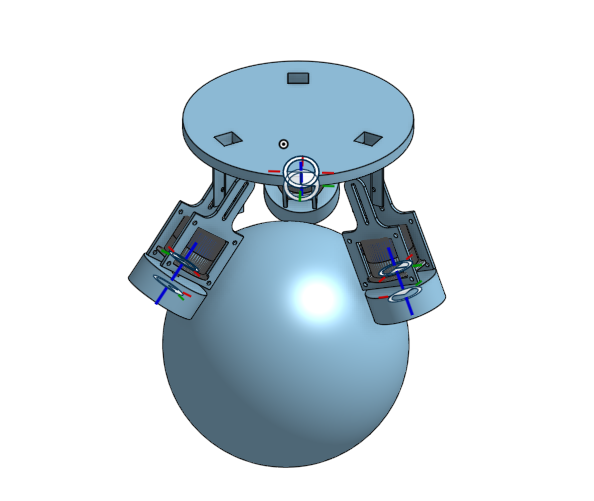
\includegraphics[width=\linewidth]{Metodologia/Figuras/ballbot.png}
        \caption{Modelo 3D}
        \label{fig:modelo_3D}
    \end{subfigure}
\end{figure}

O corpo do robô é um pequeno cilindro, onde são fixados os componentes eletrônicos. Além disso, possui partes que podem se mover para variar o ângulo das rodas e facilitar a acomodação. Essas partes também envolvem a fixação dos motores ao corpo.

\section{A modelagem matemática}
\label{sec:modelagemmatematica}

Para o projeto de controle, fez-se necessário realizar a modelagem mecânica do robô. A etapa seguinte relata como isso foi feito por meio da separação em planos 2D e obtenção das equações de movimento pelo cálculo do Lagrangiano e aplicação das equações de Euler-Lagrange. O passo a passo para realizar os cálculos foi semelhante ao presente no artigo \cite{phdthesis} e adaptado ao modelo projetado.

\subsection{Descrição do modelo}

O robô projetado foi um sistema tridimensional complexo formado por uma esfera, três rodas omnidirecionais e um corpo. Para a representação matemática simplificada, esse modelo foi dividido em três modelos planos independentes (Fig: \ref{fig:modelos_planos}).

\begin{figure}[H]
    \centering
    \begin{subfigure}[b]{0.4\textwidth}
        \centering
        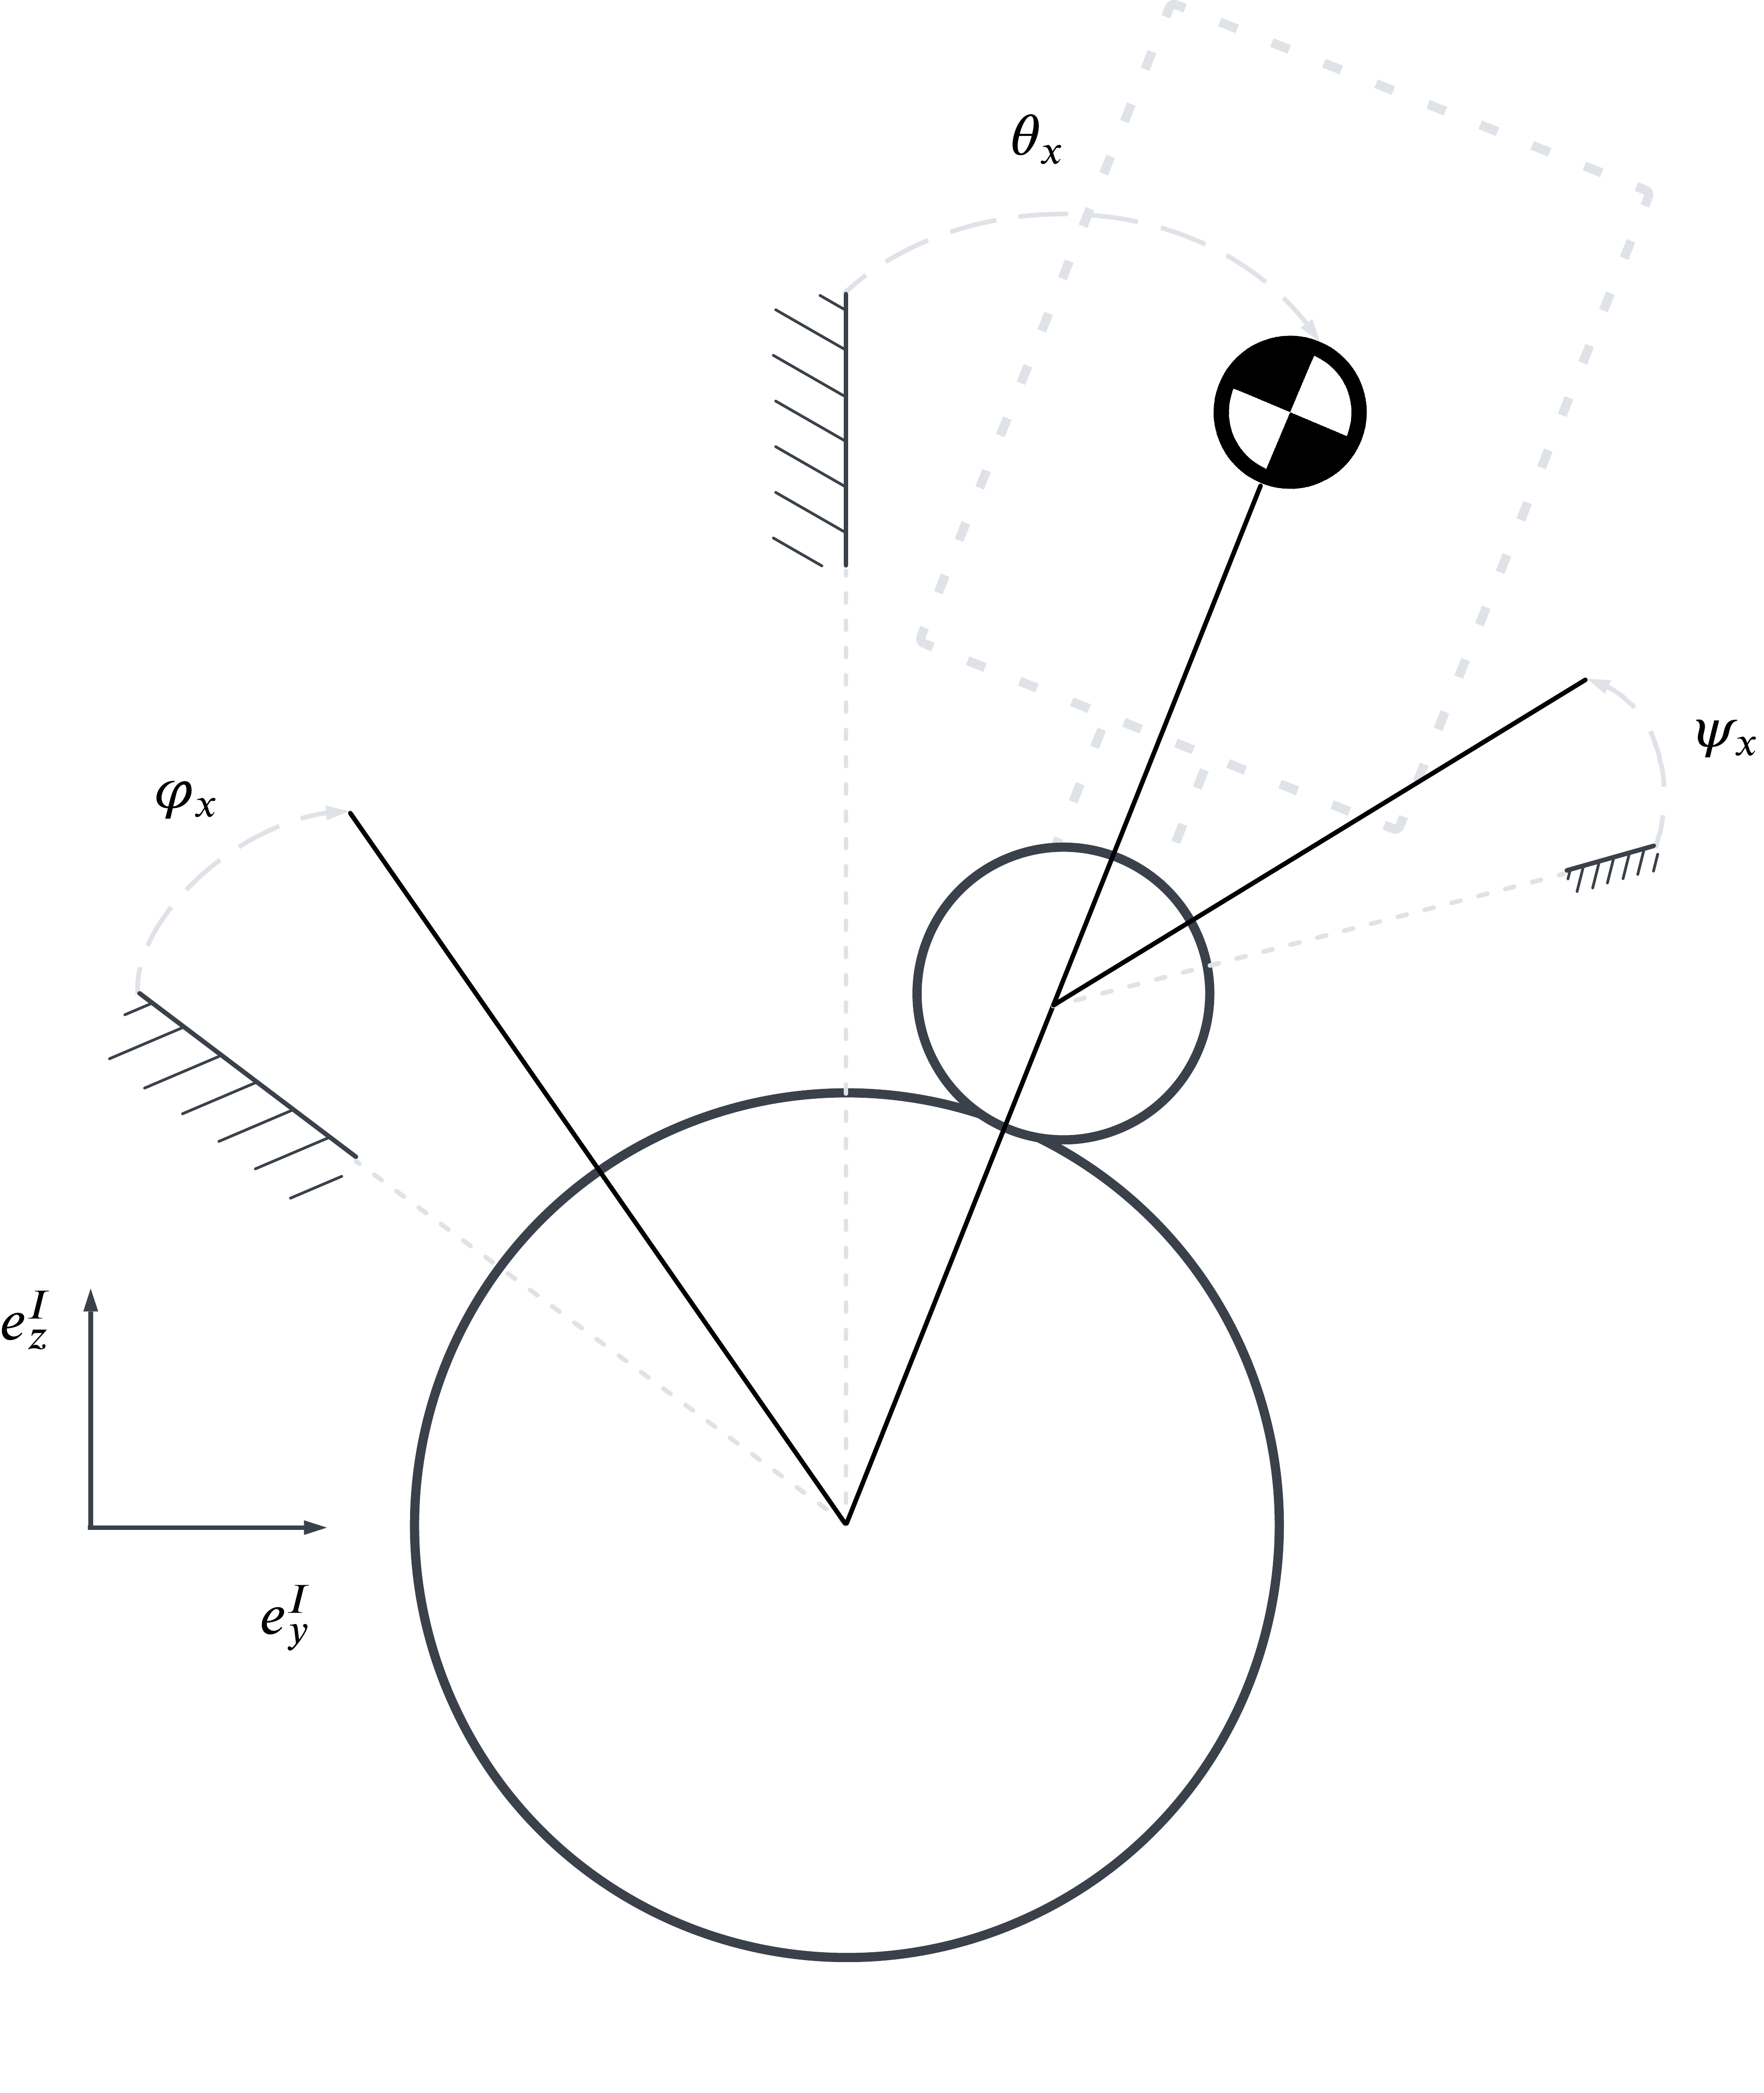
\includegraphics[width=\linewidth]{Metodologia/Figuras/modelo_plano_yz.png}
        \caption{Modelo no plano y-z}
        \label{fig:modelo_yz}
    \end{subfigure}
    \hfill
    \begin{subfigure}[b]{0.4\textwidth}
        \centering
        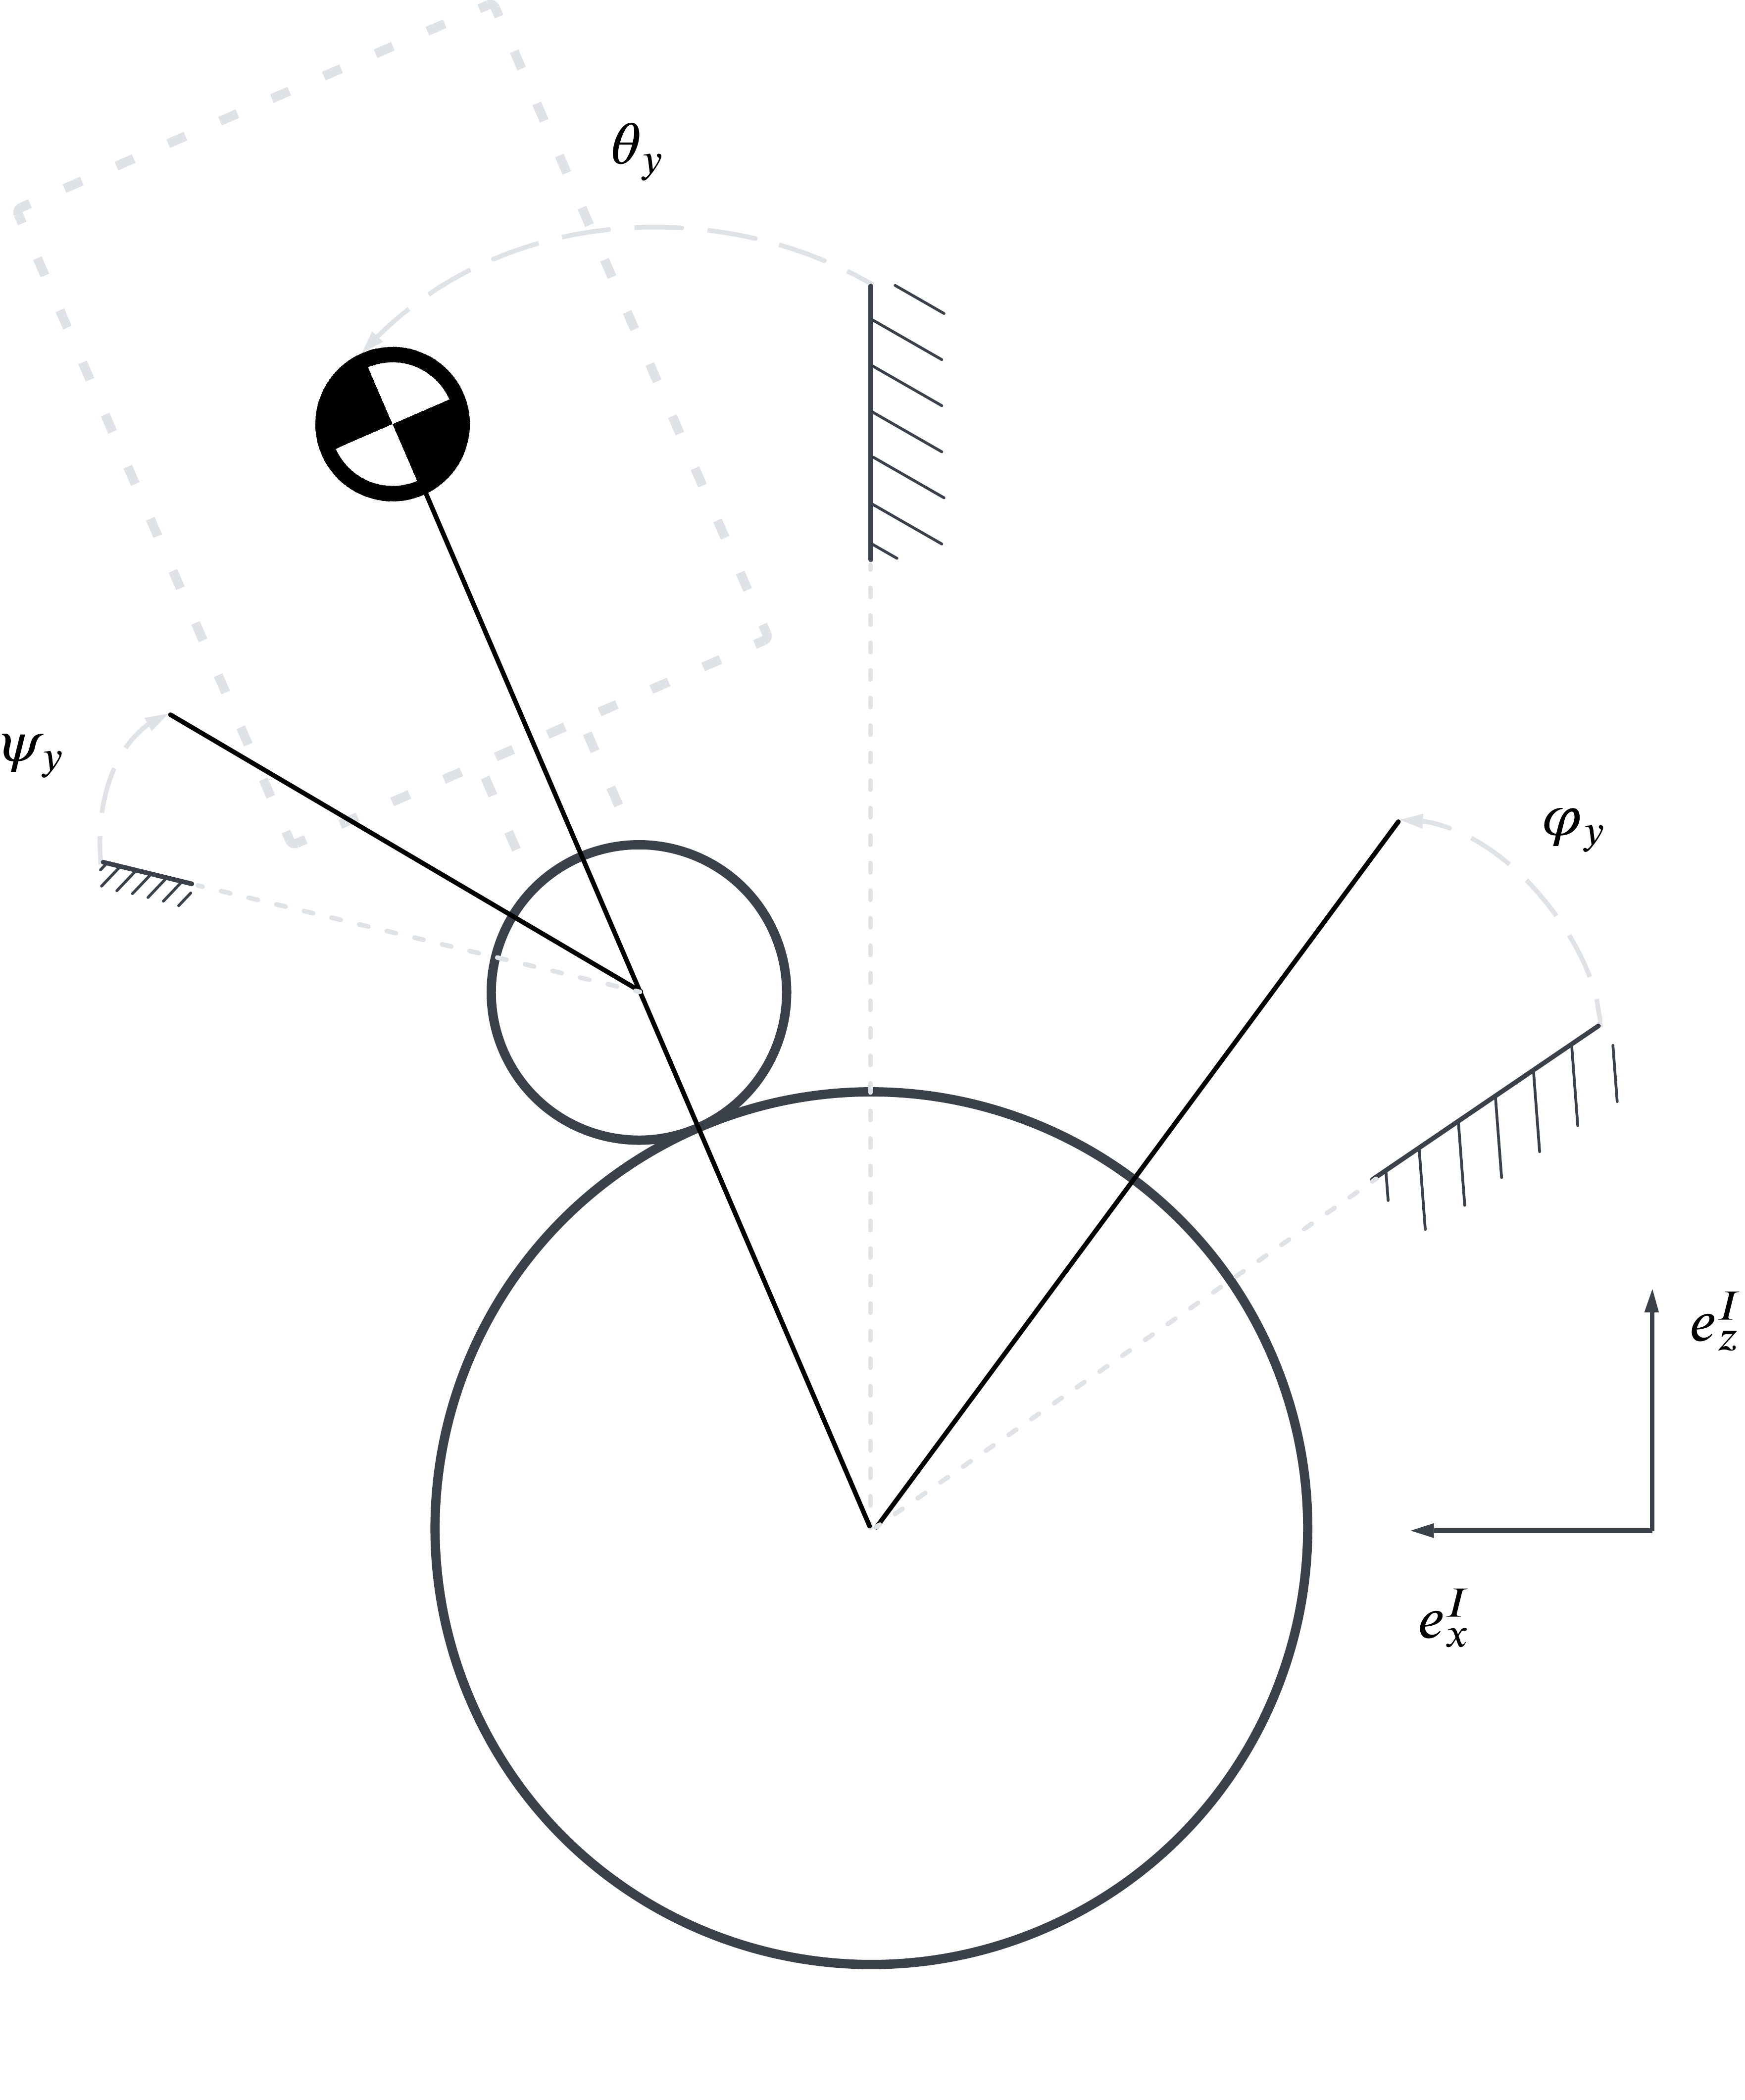
\includegraphics[width=\linewidth]{Metodologia/Figuras/modelo_plano_xz.png}
        \caption{Modelo no plano x-z}
        \label{fig:modelo_xz}
    \end{subfigure}
    \hfill
    \begin{subfigure}[b]{0.4\textwidth}
        \centering
        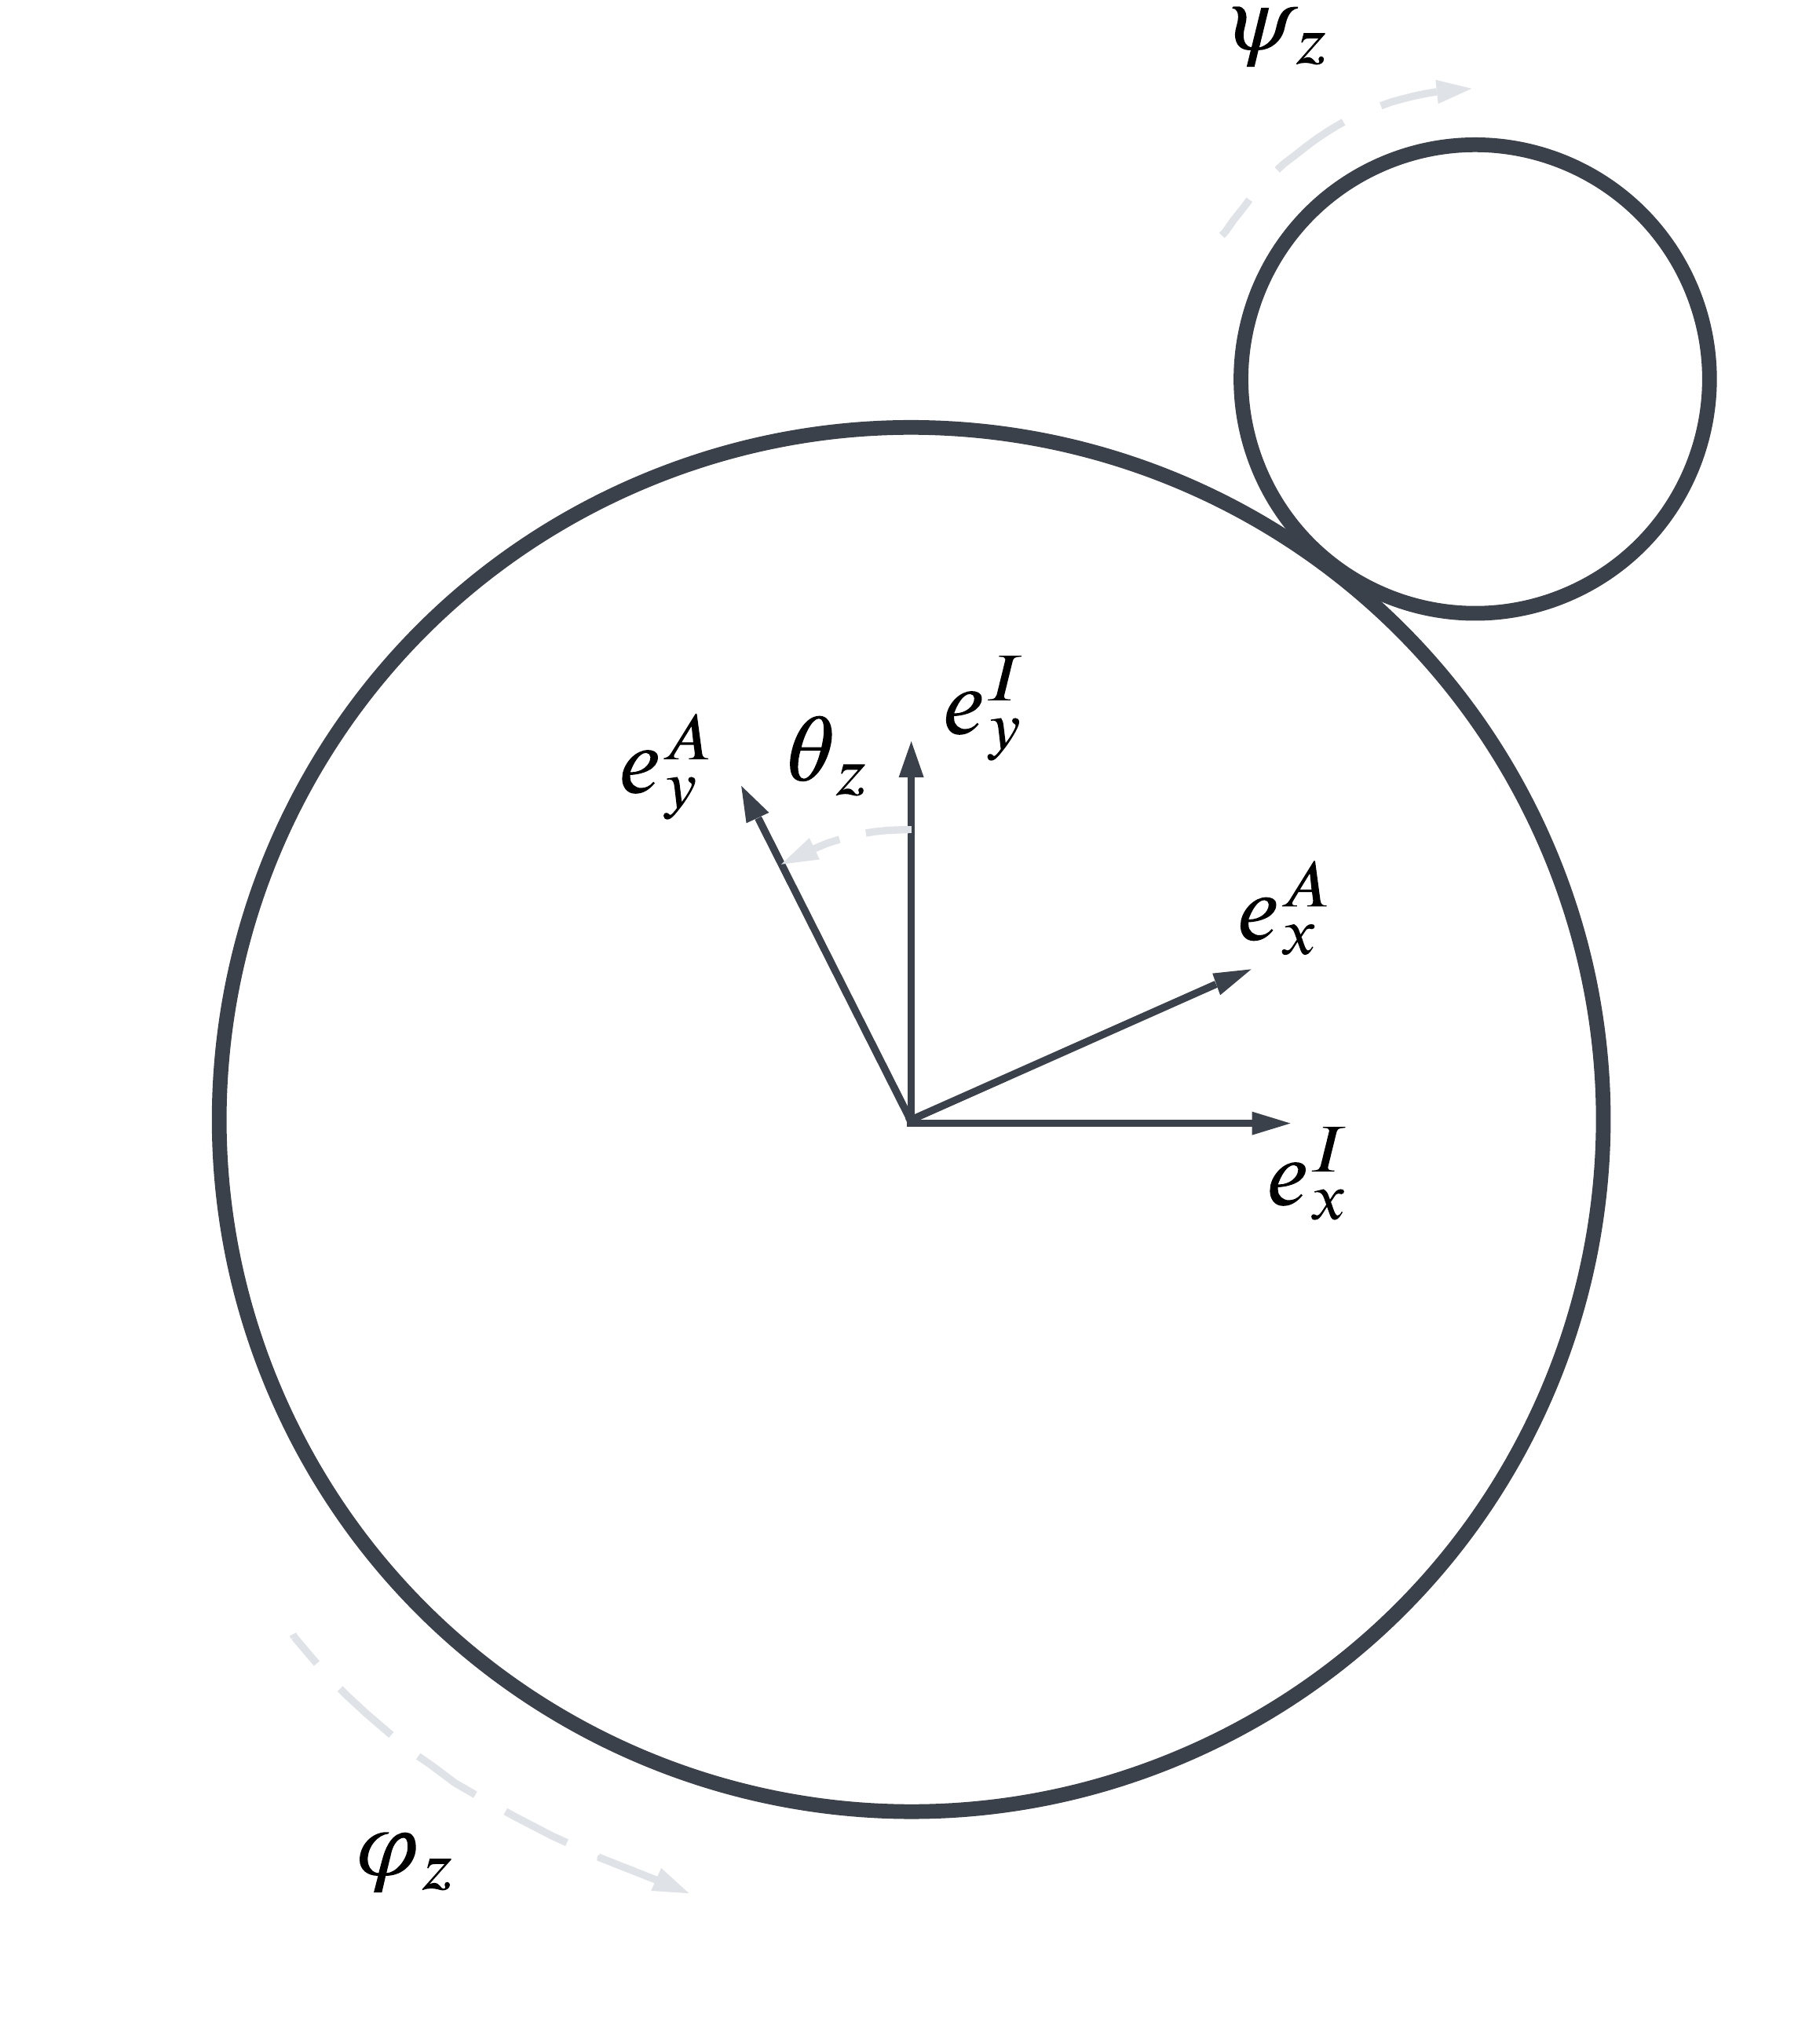
\includegraphics[width=\linewidth]{Metodologia/Figuras/modelo_plano_xy.png}
        \caption{Modelo no plano x-y}
        \label{fig:modelo_xy}
    \end{subfigure}
    \caption{Modelos nos diferentes planos}
    \label{fig:modelos_planos}
\end{figure}

Dessa forma, as três rodas omnidirecionais, que tinham o papel de movimentar o robô, foram transformadas em rodas virtuais, e cada uma foi representada em um modelo. Por causa dessa simplificação, posteriormente foram feitos cálculos para a conversão de posições e velocidades das rodas virtuais para as rodas reais.

\subsection{Suposições}

Os três modelos foram gerados a partir da subdivisão em planos do modelo tridimensional. Consequentemente, os efeitos de acoplamento entre eles foram desconsiderados. Nesse contexto, assumiu-se que o modelo representado no plano $y$-$z$ e o modelo representado no plano $x$-$z$ eram figuras espelhadas uma da outra. Por outro lado, o terceiro modelo, representado no plano $x$-$y$, tinha uma visão única, e apenas descrevia a rotação em torno do eixo \( z \) no sistema de coordenadas fixo do corpo (Fig: \ref{fig:modelo_xy}).

Ademais, com o intuito de simplificar ainda mais os cálculos e garantir a viabilidade do modelo matemático, foram adotadas as seguintes suposições:

\begin{itemize}
    \item Não há deslizamento entre a esfera e a superfície em que o robô está posicionado, assim como entre a esfera e as rodas omnidirecionais.
    \item Apenas o atrito em torno do eixo $z$, entre a esfera e a superfície, foi considerado. Todas as demais forças de atrito foram desconsideradas por serem consideradas irrelevantes.
    \item As interações entre os pontos de contato do robô são idealizadas, ou seja, não há deformações em nenhum desses pontos.
    \item A dinâmica dos motores é significativamente mais rápida do que a dinâmica de estabilização do robô, permitindo que a primeira seja tratada como praticamente instantânea em relação à segunda.
    \item A esfera está restrita a movimentos no plano horizontal, eliminando quaisquer componentes verticais.
\end{itemize}

\subsection{Parâmetros}

O robô possui alguns parâmetros estruturais que foram medidos e estão dispostos na tabela a seguir:

\begin{table}[H]
\centering
\begin{tabular}{|m{6cm}|c|c|c|}
\hline
Parâmetro & Símbolo  & Valor & Unidade de medida \\ \hline
Massa da esfera & $m_K$  & - & $kg$ \\ \hline
Massa da roda & $m_W$  & - & $kg$ \\ \hline
Massa do corpo & $m_A$  & - & $kg$ \\ \hline
Raio da esfera & $r_K$  & - & $m$ \\ \hline
Raio da roda & $r_W$  & - & $m$ \\ \hline
Distância entre o centro da esfera e o centro de massa do corpo & $l$ & - & $m$ \\ \hline
Momento de inércia da esfera & $\Theta_K$  & - & $kg \cdot m^2$ \\ \hline
Momento de inércia da roda nos planos $x$-$z$ e $y$-$z$ & $\Theta_W$  & - & $kg \cdot m^2$ \\ \hline
Momento de inércia da roda no plano $x$-$y$ & $\Theta_{W,xy}$  & - & $kg \cdot m^2$ \\ \hline
Momento de inércia do corpo & $\Theta_{A}$  & - & $kg \cdot m^2$ \\ \hline
Momento de inércia do corpo no plano $x$-$y$ & $\Theta_{A,xy}$  & - & $kg \cdot m^2$ \\ \hline
Ângulo entre o ponto de contato das rodas e o eixo z do sistema de coordenadas da esfera & $\alpha$  & - & $graus$ \\ \hline
Aceleração da gravidade & $g$  & $9,8$ & $\frac{m}{s^2}$ \\ \hline
\end{tabular}
\caption{Parâmetros estruturais}
\label{tab:tabela1}
\end{table}

\subsection{Coordenadas}

Cada um dos modelos foi completamente descrito utilizando os seguintes vetores de coordenadas mínimas:

\begin{equation}
\label{eq:1}
\begin{array}{ccc}
\vec{q_{xy}} =
\begin{bmatrix}
\varphi_z \\
\theta_z
\end{bmatrix}
& 
\vec{q_{yz}} =
\begin{bmatrix}
\varphi_x \\
\theta_x
\end{bmatrix}
& 
\vec{q_{xz}} =
\begin{bmatrix}
\varphi_y \\
\theta_y
\end{bmatrix}
\end{array}
\end{equation}

Onde:

\begin{itemize}
    \item $\varphi_{x,y,z}$: São as orientações da esfera;
    \item $\theta_{x,y,z}$: São as orientações do corpo;
    \item $\psi_{x,y,z}$: São os ângulos das rodas vituais.
\end{itemize}

\subsection{Equações de ligação}

Todas as coordenadas foram expressas utilizando os vetores de coordenadas mínimas e considerando a condição de rolamento sem deslizamento. Para um objeto circular que rola sem deslizar, o deslocamento linear do centro é diretamente proporcional à sua rotação angular, e pode ser calculado pela fórmula:

\begin{equation*}
    \begin{aligned}
        S = r \cdot \theta
    \end{aligned}
\end{equation*}

onde:

\begin{itemize}
    \item \( S \): Deslocamento linear do objeto, medido ao longo do caminho percorrido;
    \item \( r \): Raio do objeto circular;
    \item \( \theta \): Ângulo de rotação do objeto.
\end{itemize}

As coordenadas da esfera, da roda virtual e do centro de massa do corpo no plano $x$-$z$ foram definidas como:

\paragraph{Esfera:}

\begin{equation}
    \label{eq:2}
    \begin{aligned}
        x_K = r_K \cdot \varphi_y,
    \end{aligned}
\end{equation}

\begin{equation}
    \label{eq:3}
    \begin{aligned}
        z_K = 0.
    \end{aligned}
\end{equation}

\paragraph{Roda virtual:}

\begin{equation}
    \label{eq:4}
    \begin{aligned}
        x_W = (r_K \cdot \varphi_y) + (r_K + r_W) \cdot \sin{(\theta_y)},
    \end{aligned}
\end{equation}

\begin{equation}
    \label{eq:5}
    \begin{aligned}
        z_W = (r_K + r_W) \cdot \cos{(\theta_y)}.
    \end{aligned}
\end{equation}

\paragraph{Centro de massa do corpo:}

\begin{equation}
    \label{eq:6}
    \begin{aligned}
        x_A = (r_K \cdot \varphi_y) + l \cdot \sin{(\theta_y)},
    \end{aligned}
\end{equation}

\begin{equation}
    \label{eq:7}
    \begin{aligned}
        z_A = l \cdot \cos{(\theta_y)}.
    \end{aligned}
\end{equation}

Analogamente, foram encontradas as coordenadas no plano $y$-$z$:

\paragraph{Esfera:}

\begin{equation}
    \label{eq:8}
    \begin{aligned}
        y_K = r_K \cdot \varphi_x,
    \end{aligned}
\end{equation}

\begin{equation}
    \label{eq:9}
    \begin{aligned}
        z_K = 0.
    \end{aligned}
\end{equation}

\paragraph{Roda virtual:}

\begin{equation}
    \label{eq:10}
    \begin{aligned}
        y_W = (r_K \cdot \varphi_x) + (r_K + r_W) \cdot \sin{(\theta_x)},
    \end{aligned}
\end{equation}

\begin{equation}
    \label{eq:11}
    \begin{aligned}
        z_W = (r_K + r_W) \cdot \cos{(\theta_x)}.
    \end{aligned}
\end{equation}

\paragraph{Centro de massa do corpo:}

\begin{equation}
    \label{eq:12}
    \begin{aligned}
        y_A = (r_K \cdot \varphi_x) + l \cdot \sin{(\theta_x)},
    \end{aligned}
\end{equation}

\begin{equation}
    \label{eq:13}
    \begin{aligned}
        z_A = l \cdot \cos{(\theta_x)}.
    \end{aligned}
\end{equation}

No modelo do plano $x$-$z$, o ponto $A$ foi definido como o ponto de contato localizado na superfície da esfera, enquanto o ponto $B$ foi definido como o ponto de contato localizado na superfície da roda virtual. Suas velocidades, \( V_A \) e \( V_B \), foram assumidas iguais devido à condição de não deslizamento:

\begin{equation*}
    V_A = V_B \implies 
    \begin{bmatrix}
    V_{Ax} \\
    V_{Az}
    \end{bmatrix} = 
    \begin{bmatrix}
    V_{Bx} \\
    V_{Bz}
    \end{bmatrix}.
\end{equation*}

Substituindo-se os valores chegou-se em:

\begin{equation*}
    \begin{aligned}
        \begin{bmatrix}
        \dot x_K + \dot \varphi_y \cdot r_k \cdot \cos(\theta_y) \\
        \dot \varphi_y \cdot r_K \cdot \sin(\theta_y)
        \end{bmatrix}=
        \begin{bmatrix}
        \dot x_K + (r_K + r_W) \cdot \cos(\theta_y) \cdot \dot \theta_y + \dot \psi_y \cdot r_W \cdot \cos(\theta_y) \\
        - (r_K + r_W) \cdot \sin(\theta_y) \cdot \dot \theta_y + \dot \psi_y \cdot r_W \cdot \sin(\theta_y)
        \end{bmatrix}.
    \end{aligned}
\end{equation*}

Ao se isolar $\dot \psi_y$, obteve-se:

\begin{equation}
    \label{eq:14}
    \begin{aligned}
        \dot \psi_y = \frac{r_K}{r_W} \cdot (\dot \varphi_y - \dot \theta_y) - \dot \theta_y
    \end{aligned}.
\end{equation}

Analogamente, no plano $y$-$z$, foi obtido:

\begin{equation}
    \label{eq:15}
    \begin{aligned}
        \dot \psi_x = \frac{r_K}{r_W} \cdot (\dot \varphi_x - \dot \theta_x) - \dot \theta_x
    \end{aligned}.
\end{equation}

Por fim, utilizando-se o modelo no plano $x$-$y$, as velocidades \( V_A \) e \( V_B \) foram definidas como:

\begin{equation*}
    V_A = 
    \begin{bmatrix}
    V_{Ax} \\
    V_{Ay}
    \end{bmatrix}, \quad 
    V_B = 
    \begin{bmatrix}
    V_{Bx} \\
    V_{By}
    \end{bmatrix}.
\end{equation*}

Assumiu-se novamente \( V_A = V_B \) e se substituíram os valores, obtendo-se:

\begin{equation*}
    \begin{aligned}
        \begin{bmatrix}
        r_K \cdot \sin(\alpha) \cdot \dot \varphi_z \cdot \cos(\theta_z) \\
        r_K \cdot \sin(\alpha) \cdot \dot \varphi_z \cdot \sin(\theta_z)
        \end{bmatrix}=
        \begin{bmatrix}
        r_K \cdot \sin(\alpha) \cdot \dot \theta_z \cdot \cos(\theta_z) + r_W \cdot \dot \psi_z \cdot \cos(\theta_z)\\
        r_K \cdot \sin(\alpha) \cdot \dot \theta_z \cdot \sin(\theta_z) + r_W \cdot \dot \psi_z \cdot \sin(\theta_z)
        \end{bmatrix}.
    \end{aligned}
\end{equation*}

Isolando \( \dot{\psi}_z \), foi obtido:

\begin{equation}
    \label{eq:16}
    \begin{aligned}
        \dot \psi_z = \frac{r_K}{r_W} \cdot \sin(\alpha) \cdot (\dot \varphi_z - \dot \theta_z)
    \end{aligned}.
\end{equation}

\subsection{Energias}

O cálculo das energias potenciais e cinéticas é essencial para a modelagem utilizando o método de Euler-Lagrange. Portanto, para cada modelo planar, esses valores foram calculados como demonstrado a seguir.

\subsubsection{Plano y-z}

\paragraph{Esfera: Energia potencial}

O referencial escolhido se localizava no centro da esfera, logo, a energia potencial nessa situação era nula:

\begin{equation*}
    \begin{aligned}
        V_{K,yz} = 0
    \end{aligned}
\end{equation*}

\paragraph{Esfera: Energia cinética}

A energia cinética foi obtida por meio da soma da parte translacional e da parte rotacional:

\begin{equation*}
    \begin{aligned}
        T_{K,yz} & =\frac{1}{2} \cdot m_K \cdot (r_K \cdot \dot\varphi_x)^2 + \frac{1}{2} \cdot \Theta_K \cdot \dot\varphi_x^2
    \end{aligned}
\end{equation*}

\paragraph{Roda: Energia potencial}

\begin{equation*}
    \begin{aligned}
        V_{W,yz} & = m_W \cdot g \cdot (r_K + r_W) \cdot \cos{(\theta_x)}
    \end{aligned}
\end{equation*}

\paragraph{Roda: Energia cinética}

\begin{equation*}
    \begin{aligned}
        T_{W,yz} & = \frac{1}{2} \cdot m_W \cdot 
        \begin{bmatrix}
            \dot x_W \\
            \dot y_W \\
            \dot z_W
        \end{bmatrix}^T
        \cdot
        \begin{bmatrix}
            \dot x_W \\
            \dot y_W \\
            \dot z_W
        \end{bmatrix}
        +
        \frac{1}{2} \cdot \Theta_W \cdot \dot {\psi_x}^2
    \end{aligned}
\end{equation*}

Os valores de $x_W$, $y_W$ e $z_W$ são:

\begin{equation*}
\scalebox{0.85}{$
    \begin{aligned}
        \begin{bmatrix}
            x_W \\
            y_W \\
            z_W
        \end{bmatrix} 
        & =
        \begin{bmatrix}
            0 \\
            (\varphi_x \cdot r_K ) + (r_K + r_W) \cdot \sin(\theta_x) \\
            (r_K + r_W) \cdot \cos(\theta_x)
        \end{bmatrix}
        \implies
        \begin{bmatrix}
            \dot x_W \\
            \dot y_W \\
            \dot z_W
        \end{bmatrix}
        & =
        \begin{bmatrix}
            0 \\
            (\dot \varphi_x \cdot r_K ) + (r_K + r_W) \cdot \cos({\theta_x}) \cdot \dot \theta_x \\
            - (r_K + r_W) \cdot \sin({\theta_x}) \cdot \dot \theta_x
        \end{bmatrix}.
    \end{aligned}
    $}
\end{equation*}.

Ao substituir esse resultado na equação anterior, obteve-se:

\begin{equation*}
    \scalebox{0.65}{$
        \begin{aligned}
            T_{W,yz} = \frac{1}{2} \cdot m_W \cdot \Big[ (\dot{\varphi}_x \cdot r_K)^2 + 2 \cdot (\dot{\varphi}_x \cdot r_K) \cdot (r_K + r_W) \cdot \cos(\theta_x) \cdot \dot{\theta}_x + (r_K + r_W)^2 \cdot \dot{\theta}_x^2 \Big] + \frac{1}{2} \cdot \Theta_W \cdot \bigg(\frac{r_K}{r_W} \cdot (\dot{\varphi}_x - \dot{\theta}_x) - \dot{\theta}_x \bigg)^2
        \end{aligned}
    $}
\end{equation*}


\paragraph{Corpo: Energia potencial}

\begin{equation*}
    \begin{aligned}
        V_{A,yz} & = m_A \cdot g \cdot l \cdot \cos{(\theta_x)}
    \end{aligned}
\end{equation*}

\paragraph{Corpo: Energia cinética}

\begin{equation*}
    \begin{aligned}
        T_{A,yz} & = \frac{1}{2} \cdot m_A \cdot 
        \begin{bmatrix}
            \dot x_A \\
            \dot y_A \\
            \dot z_A
        \end{bmatrix}^T
        \cdot
        \begin{bmatrix}
            \dot x_A \\
            \dot y_A \\
            \dot z_A
        \end{bmatrix}
        +
        \frac{1}{2} \cdot \Theta_A \cdot \dot {\theta_x}^2
    \end{aligned}
\end{equation*}

Os valores de $x_A$, $y_A$ e $z_A$ são:

\begin{equation*}
    \begin{aligned}
        \begin{bmatrix}
            x_A \\
            y_A \\
            z_A
        \end{bmatrix} 
        & =
        \begin{bmatrix}
            0 \\
            (\varphi_x \cdot r_K ) + l \cdot \sin(\theta_x) \\
            l \cdot \cos(\theta_x)
        \end{bmatrix}
        \implies
        \begin{bmatrix}
            \dot x_A \\
            \dot y_A \\
            \dot z_A
        \end{bmatrix}
        & =
        \begin{bmatrix}
            0 \\
            (\dot \varphi_x \cdot r_K ) + l \cdot \cos({\theta_x}) \cdot \dot \theta_x \\
            - l \cdot \sin({\theta_x}) \cdot \dot \theta_x
        \end{bmatrix}.
    \end{aligned}
\end{equation*}.

Ao substituir esse resultado na equação anterior, foi obtido:

\begin{equation*}
    \begin{aligned}
        T_{A,yz} = \frac{1}{2} \cdot m_A \cdot \Big[ (\dot{\varphi}_x \cdot r_K)^2 + 2 \cdot (\dot{\varphi}_x \cdot r_K) \cdot l \cdot \cos(\theta_x) \cdot \dot{\theta}_x + l^2 \cdot \dot{\theta}_x^2 \Big] + \frac{1}{2} \cdot \Theta_A \cdot \dot \theta_x^2
    \end{aligned}
\end{equation*}

\subsubsection{Plano x-z}

As equações do plano x-z são análogas às equações do plano y-z.

\paragraph{Esfera: Energia potencial}

\begin{equation*}
    \begin{aligned}
        V_{K,xz} = 0
    \end{aligned}
\end{equation*}

\paragraph{Esfera: Energia cinética}

\begin{equation*}
    \begin{aligned}
        T_{K,xz} & = \frac{1}{2} \cdot m_K \cdot (r_K \cdot \dot\theta_y)^2 + \frac{1}{2} \cdot \Theta_K \cdot \dot\theta_y^2
    \end{aligned}
\end{equation*}

\paragraph{Roda: Energia potencial}

\begin{equation*}
    \begin{aligned}
        V_{W,xz} & = m_W \cdot g \cdot (r_K + r_W) \cdot \cos{(\theta_y)}
    \end{aligned}
\end{equation*}

\paragraph{Roda: Energia cinética}

\begin{equation*}
    \scalebox{0.65}{$
    \begin{aligned}
        T_{W,xz} = \frac{1}{2} \cdot m_W \cdot \Big[ (\dot{\varphi}_y \cdot r_K)^2 
        + 2 \cdot (\dot{\varphi}_y \cdot r_K) \cdot (r_K + r_W) \cdot \cos(\theta_y) \cdot \dot{\theta}_y + (r_K + r_W)^2 \cdot \dot{\theta}_y^2 \Big] + \frac{1}{2} \cdot \Theta_W \cdot \bigg(\frac{r_K}{r_W} \cdot (\dot{\varphi}_y - \dot{\theta}_y) - \dot{\theta}_y \bigg)^2
    \end{aligned}
    $}
\end{equation*}

\paragraph{Corpo: Energia potencial}

\begin{equation*}
    \begin{aligned}
        V_{A,xz} & = m_A \cdot g \cdot l \cdot \cos{(\theta_y)}
    \end{aligned}
\end{equation*}

\paragraph{Corpo: Energia cinética}

\begin{equation*}
    \begin{aligned}
        T_{A,xz} = \frac{1}{2} \cdot m_A \cdot \Big[ (\dot{\varphi}_y \cdot r_K)^2 + 2 \cdot (\dot{\varphi}_y \cdot r_K) \cdot l \cdot \cos(\theta_y) \cdot \dot{\theta}_y + l^2 \cdot \dot{\theta}_y^2 \Big] + \frac{1}{2} \cdot \Theta_A \cdot \dot \theta_y^2
    \end{aligned}
\end{equation*}

\subsubsection{Plano x-y}

\paragraph{Esfera: Energia cinética}

\begin{equation*}
    \begin{aligned}
        T_{K,xy} & = \frac{1}{2} \cdot \Theta_K \cdot \dot {\varphi_z}^2 
    \end{aligned}
\end{equation*}

\paragraph{Roda: Energia cinética}

\begin{equation*}
    \begin{aligned}
        T_{W,xy} & = \frac{1}{2} \cdot \Theta_{W,xy} \cdot \dot {\psi_z}^2 
    \end{aligned}
\end{equation*}

\paragraph{Corpo: Energia cinética}

\begin{equation*}
    \begin{aligned}
        T_{A,xy} & = \frac{1}{2} \cdot \Theta_{A,xy} \cdot \dot {\theta_z}^2 
    \end{aligned}
\end{equation*}

\subsection{Torques externos}

As forças não-potenciais \( \vec{f}_{NP} \) representam as forças externas atuando em um sistema. Neste caso, o torque do motor \( T_x \), ou seja, a entrada do sistema, é uma força não potencial. O torque do motor afeta diretamente a coordenada \( \psi_x \). Usando a equação \ref{eq:15}, o efeito do torque do motor nas coordenadas mínimas pode ser expresso como:

\begin{equation}
\label{eq:17}
\vec{f}_{NP,yz1} = 
\begin{bmatrix}
\frac{r_K}{r_W} \cdot T_x \\
-\left(1 + \frac{r_K}{r_W}\right) T_x
\end{bmatrix}
\end{equation}

O torque oposto que atua na coordenada \( \vartheta_x \) do corpo é expresso como:

\begin{equation}
\label{eq:18}
\vec{f}_{NP,yz2} =
\begin{bmatrix}
0 \\
T_x
\end{bmatrix}
\end{equation}

A força total não potencial é então a soma de \( \vec{f}_{NP,yz1} \) e \( \vec{f}_{NP,yz2} \). Um procedimento semelhante é aplicado no plano \( x \)-\( y \). Neste modelo, uma força adicional de atrito \( T_f \) atua em \( \varphi_z \), assim como na rotação da bola:

\begin{equation}
\label{eq:19}
\vec{f}_{NP,xy} =
\begin{bmatrix}
-T_f + \frac{r_K}{r_W} \sin{\alpha} \cdot T_z \\
-\frac{r_K}{r_W} \sin{\alpha} \cdot T_z + T_z
\end{bmatrix}
\end{equation}

\subsection{Equações de movimento}

\begin{equation*}
    \frac{d}{dt} \left( \frac{\partial T}{\partial \dot{\vec{q}}} \right)^T - \left( \frac{\partial T}{\partial \vec{q}} \right)^T + \left( \frac{\partial V}{\partial \vec{q}} \right)^T - \vec{f}_{NP} = 0.
\end{equation*}

$T$ e $V$ são, respectivamente, as energias cinéticas e as energias potenciais.

\begin{equation*}
    T = T_K + T_W + T_A
\end{equation*}
\begin{equation*}
    V = V_K + V_W + V_A
\end{equation*}

As equações de movimento do plano $y$-$z$ podem ser escritas na forma matricial.

\begin{equation*}
M_x(\vec{q}, \dot{\vec{q}}) \ddot{\vec{q}} + C_x(\vec{q}, \dot{\vec{q}}) + G_x(\vec{q}) = f_{NP}
\end{equation*}

As matrizes de inércia, $M_x$, de forças de Coriolis, $C_x$, e de forças gravitacionais, $G_x$, são:

\begin{equation*}
    \begin{aligned}
    M_x &= 
    \begin{bmatrix}
    m_{\text{tot}} r_K^2 + \Theta_K + \left( \frac{r_K}{r_W} \right)^2 \Theta_W & -\frac{r_K}{r_W^2} r_{\text{tot}} \Theta_W + \gamma r_K \cos \vartheta_x \\
    -\frac{r_K}{r_W^2} r_{\text{tot}} \Theta_W + \gamma r_K \cos \vartheta_x & \frac{r_{\text{tot}}^2}{r_W^2} \Theta_W + \Theta_A + m_A l^2 + m_W r_{\text{tot}}^2
    \end{bmatrix}
    \\
    C_x &= 
    \begin{bmatrix}
    -r_K \gamma \sin \vartheta_x \dot{\vartheta}_x^2 \\
    0
    \end{bmatrix}
    \\
    G_x &= 
    \begin{bmatrix}
    0 \\
    -g \sin \vartheta_x \gamma
    \end{bmatrix}
    \end{aligned}
\end{equation*}

Onde:

\begin{equation*}
    \begin{aligned}
        m_{\text{tot}} &= m_K + m_A + m_W \\
        r_{\text{tot}} &= r_K + r_W \\
        \gamma &= l \cdot m_A + (r_K + r_W) m_W
    \end{aligned}
\end{equation*}

A resolução das equações de Lagrange no plano $x$-$y$ para as coordenadas $\ddot{\varphi}_z$ e $\ddot{\vartheta}_z$ produziu:

\begin{equation}
    \label{eq:17}
    \begin{aligned}
    \ddot{\varphi}_z &= 
    -\frac{
    \left( r_W^2 \Theta_{A,xy} + r_K^2 \Theta_{W,xy} \sin^2 \alpha \right) \cdot T_f + r_K r_W \Theta_{A,xy} \sin \alpha \cdot T_z
    }{
    r_W^2 \Theta_{A,xy} \Theta_K + r_K^2 \left( \Theta_{A,xy} + \Theta_K \right) \Theta_{W,xy} \sin^2 \alpha
    }
    \end{aligned}
\end{equation}

\begin{equation}
    \label{eq:18}
    \begin{aligned}
    \ddot{\vartheta}_z &= 
    -\frac{
    r_K \sin \alpha \left( r_K \Theta_{W,xy} \sin \alpha \cdot T_f + r_W \Theta_K \cdot T_z \right)
    }{
    r_W^2 \Theta_{A,xy} \Theta_K + r_K^2 \left( \Theta_{A,xy} + \Theta_K \right) \Theta_{W,xy} \sin^2 \alpha
    }
    \end{aligned}
\end{equation}

Para determinar a força de atrito, considerou-se que a bola permanece constantemente aderida ao solo, satisfazendo a condição de aderência $\ddot\varphi=0$. Assim, com base na equação \ref{eq:17}, $T_f$ foi expresso da seguinte maneira:

\begin{equation*}
    T_f = \frac{r_K r_W \Theta_{A,xy} \sin \alpha \cdot T_z}{r_W^2 \Theta_{A,xy} + r_K^2 \Theta_{W,xy} \sin^2 \alpha}
\end{equation*}

\subsection{Conversão de torques}

Os modelos planares utilizam uma roda virtual para atuar no sistema. O sistema real possui uma estrutura de atuação que difere significativamente daquela assumida no modelo planar. Como um controlador projetado para o modelo planar será implementado no sistema real, é necessário calcular conversões. Para que seja possível controlar o sistema real, os torques nos motores virtuais devem ser convertidos nos torques dos motores reais.

A visão lateral e a visão superior do modelo real estão definidas nas figuras abaixo:

\begin{figure}[H]
    \centering
    \begin{subfigure}[b]{0.4\textwidth}
        \centering
        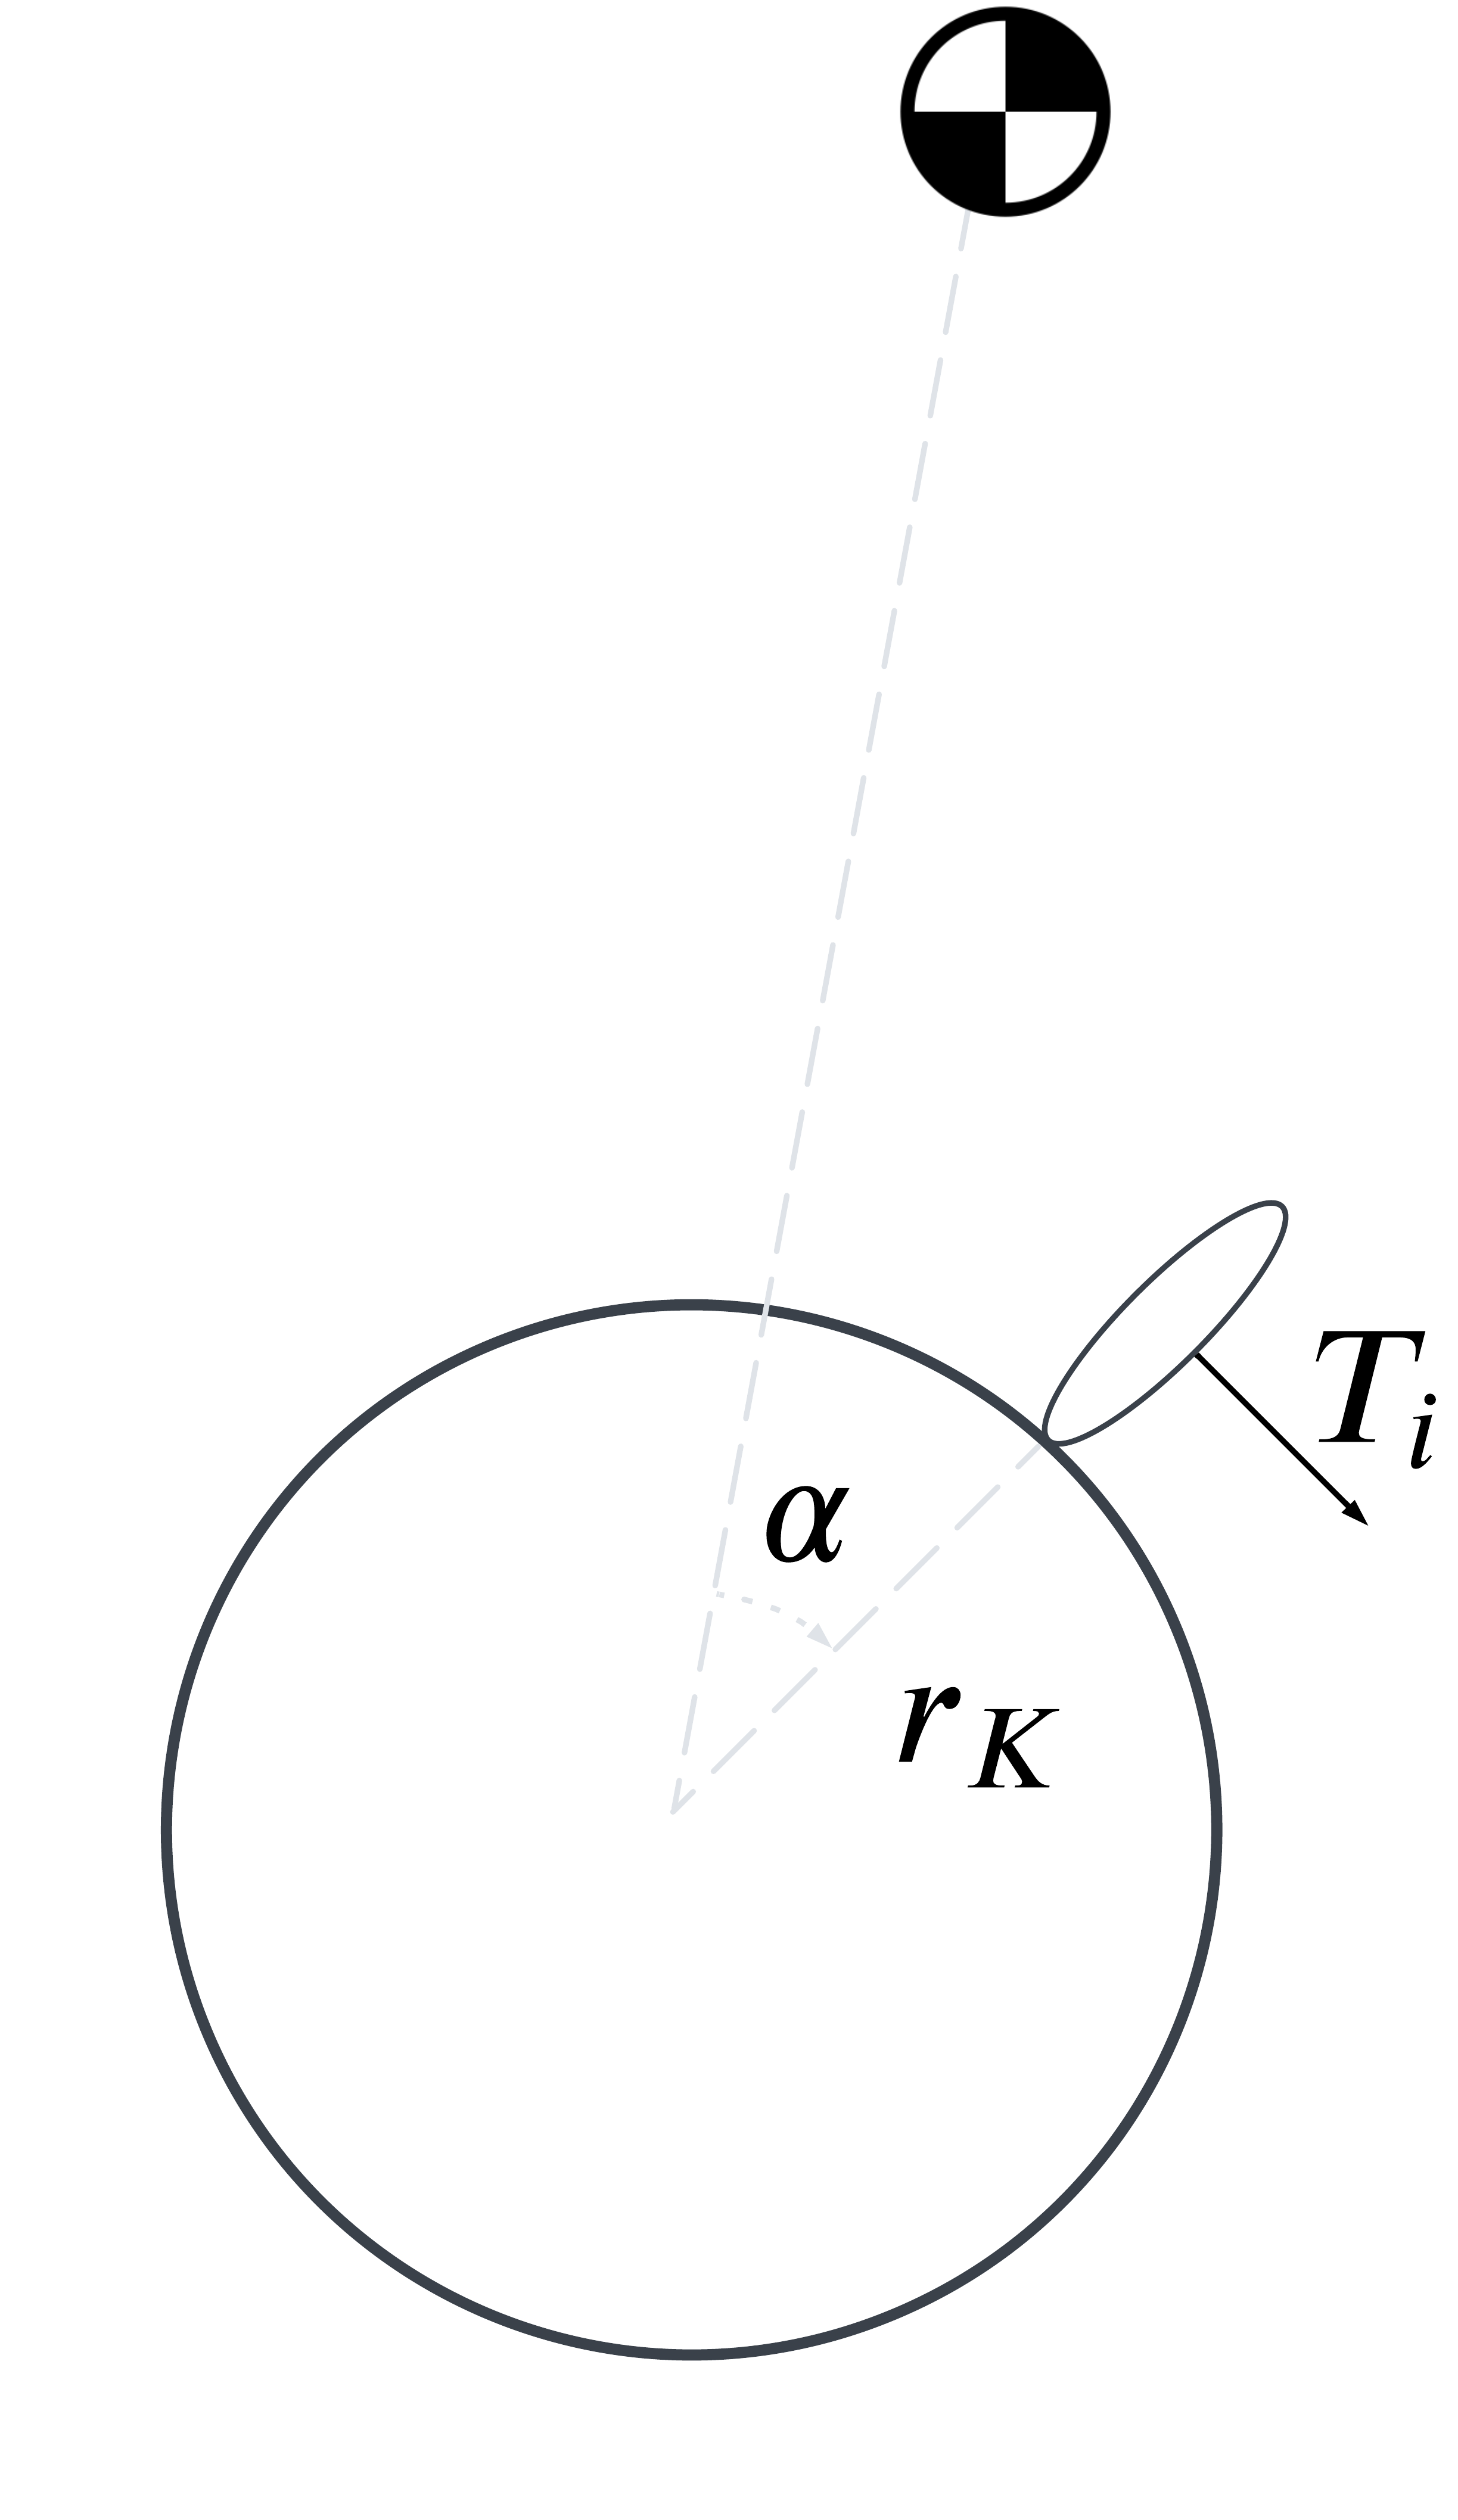
\includegraphics[width=\linewidth]{Metodologia/Figuras/torque_side.png}
        \caption{Modelo real visto de lado}
        \label{fig:torques_lado}
    \end{subfigure}
    \hfill
    \begin{subfigure}[b]{0.4\textwidth}
        \centering
        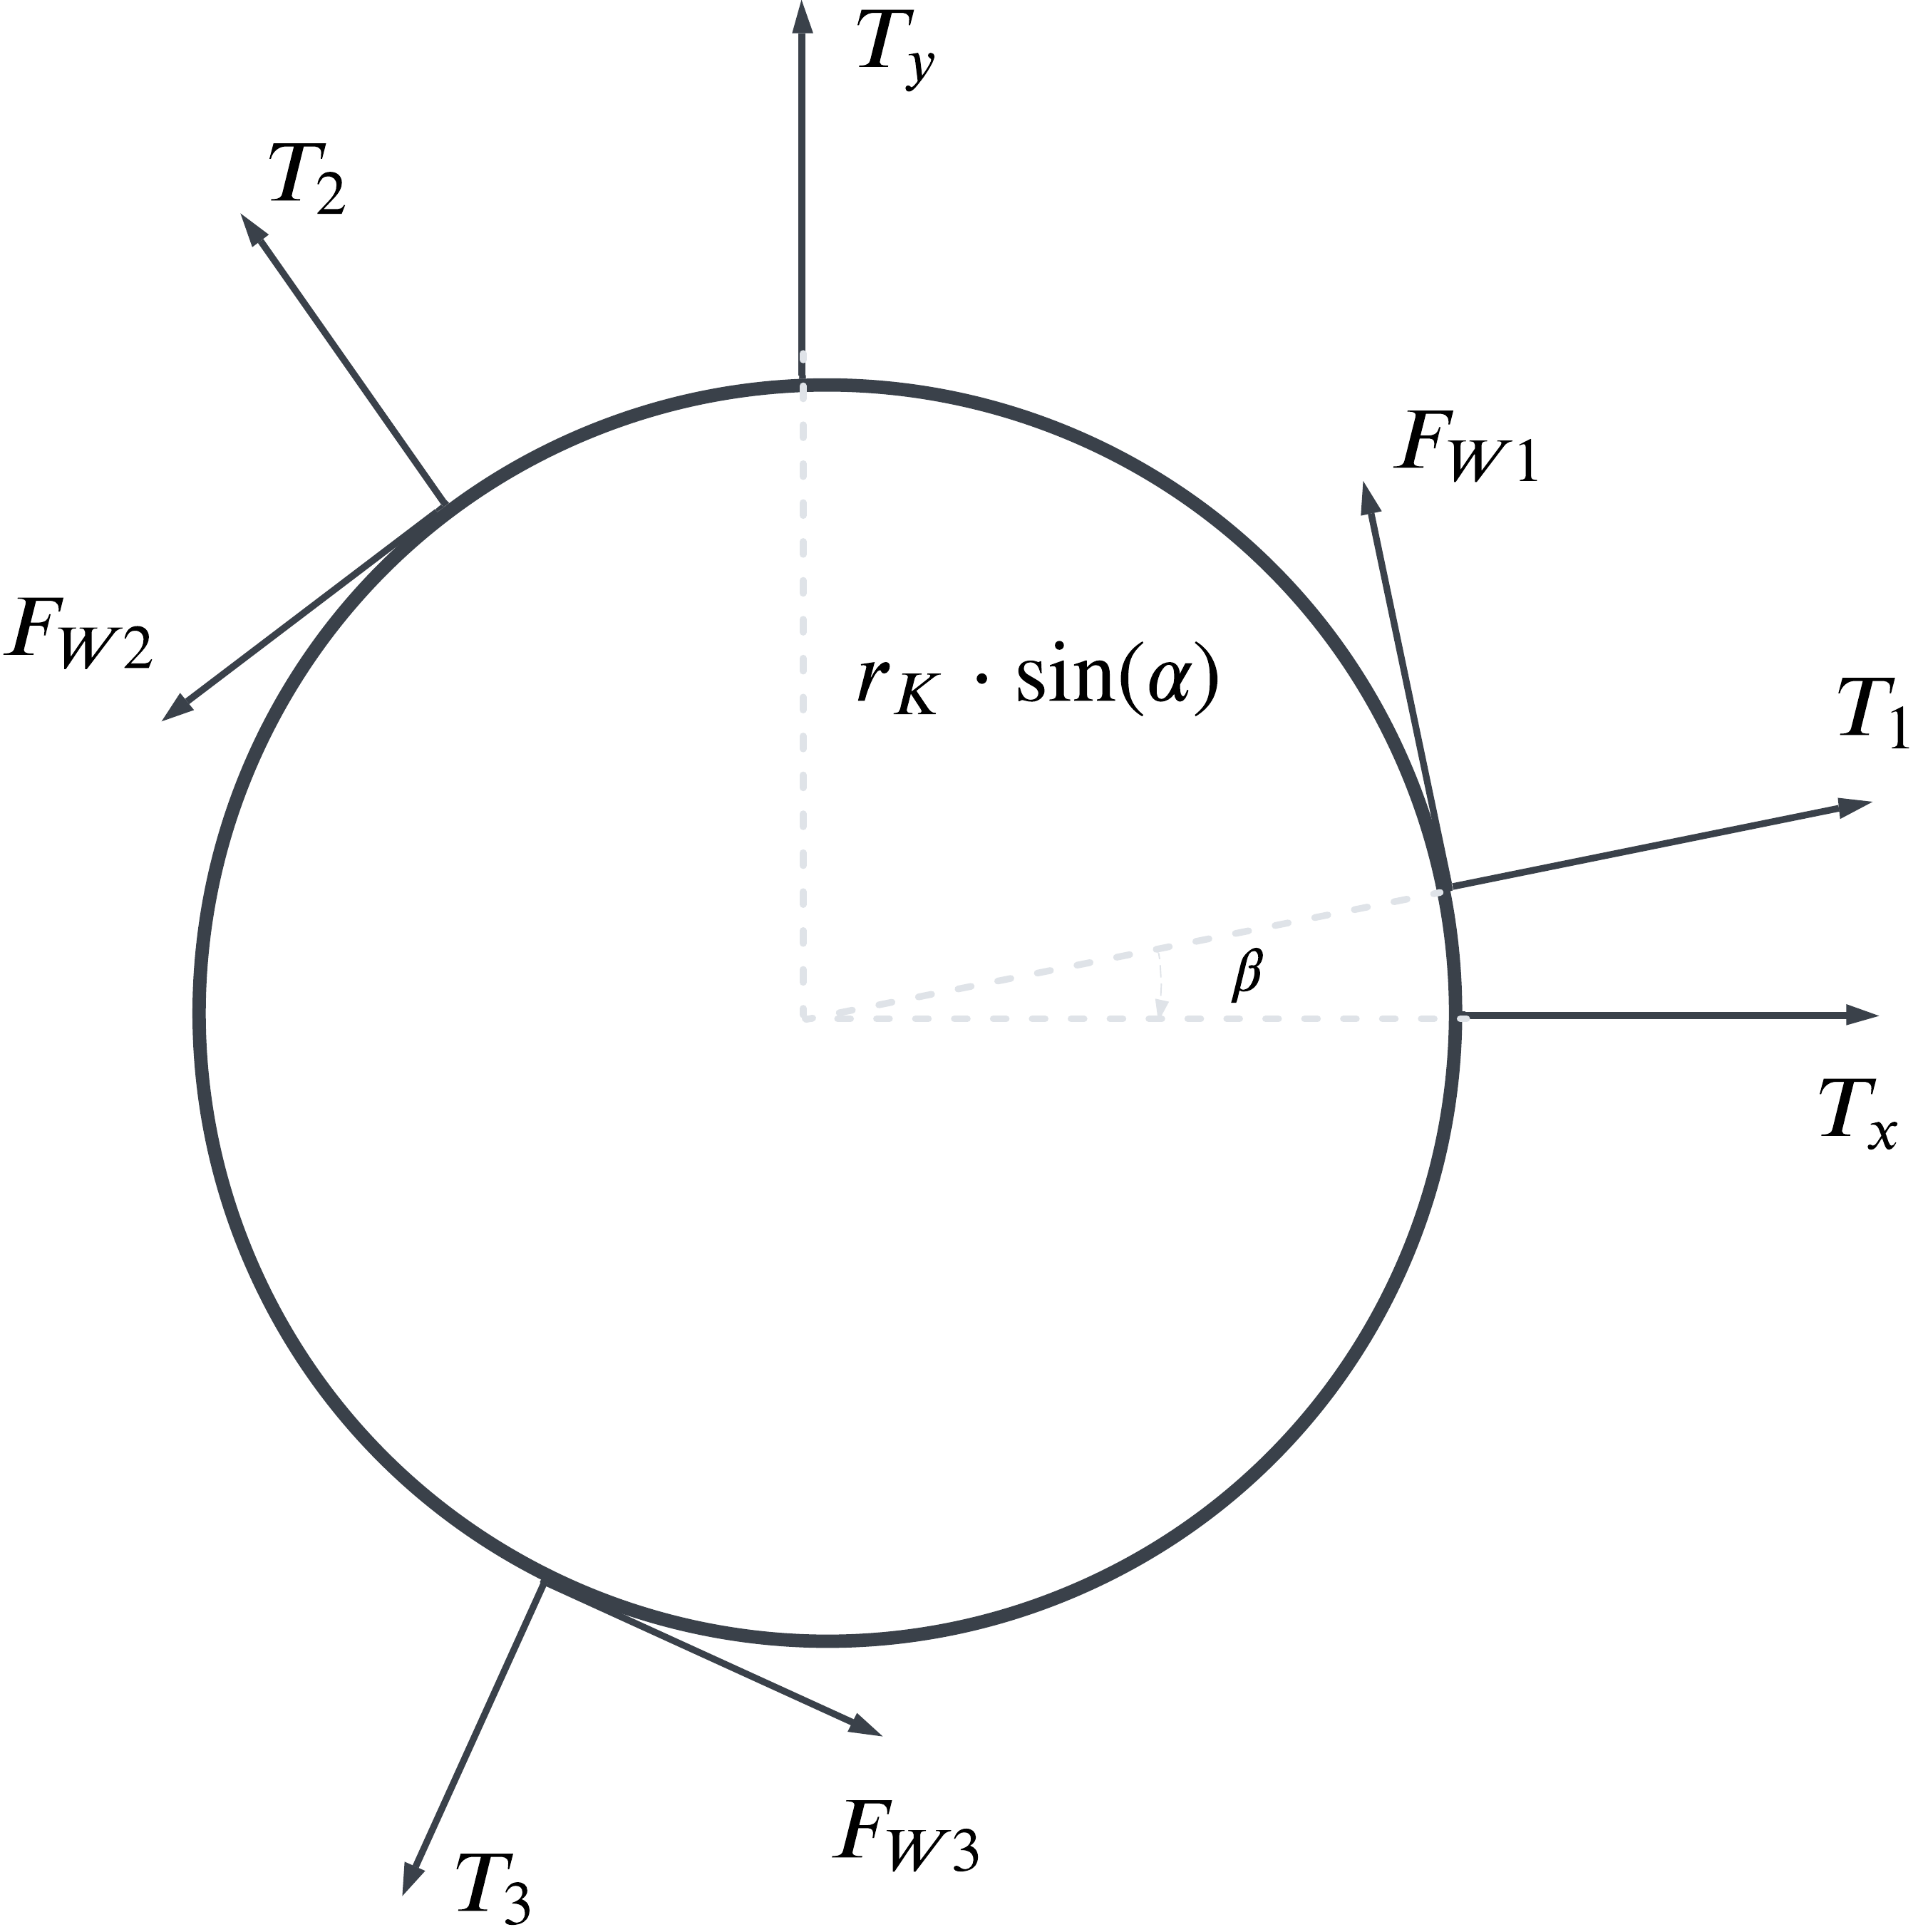
\includegraphics[width=\linewidth]{Metodologia/Figuras/torque_up.png}
        \caption{Modelo real visto de cima}
        \label{fig:torques_cima}
    \end{subfigure}
\end{figure}

Usando esses modelos, obteve-se as forças tangentes provocadas pelo torque dos motores:

\begin{equation}
    \begin{aligned}
    F_{W,1} &= \frac{T_1}{r_W} 
    \begin{bmatrix}
    -\sin \beta \\
    \cos \beta \\
    0
    \end{bmatrix}, \\
    F_{W,2} &= \frac{T_2}{r_W} 
    \begin{bmatrix}
    -\sin \left( \beta + \frac{2}{3}\pi \right) \\
    \cos \left( \beta + \frac{2}{3}\pi \right) \\
    0
    \end{bmatrix}, \\
    F_{W,3} &= \frac{T_3}{r_W} 
    \begin{bmatrix}
    -\sin \left( \beta - \frac{2}{3}\pi \right) \\
    \cos \left( \beta - \frac{2}{3}\pi \right) \\
    0
    \end{bmatrix}.
    \end{aligned}
\end{equation}

Os braços de alavanca também foram obtidos:

\begin{equation}
    \begin{aligned}
        r_{KW,1} &= r_K \cdot 
        \begin{bmatrix}
        \cos \beta \sin \alpha \\
        \sin \beta \sin \alpha \\
        \cos \alpha
        \end{bmatrix}, \\
        r_{KW,2} &= r_K \cdot 
        \begin{bmatrix}
        \cos \left( \beta + \frac{2}{3}\pi \right) \sin \alpha \\
        \sin \left( \beta + \frac{2}{3}\pi \right) \sin \alpha \\
        \cos \alpha
        \end{bmatrix}, \\
        r_{KW,3} &= r_K \cdot 
        \begin{bmatrix}
        \cos \left( \beta - \frac{2}{3}\pi \right) \sin \alpha \\
        \sin \left( \beta - \frac{2}{3}\pi \right) \sin \alpha \\
        \cos \alpha
        \end{bmatrix}.
    \end{aligned}
\end{equation}

Ainda, obteve-se as forças tangentes nos modelos planares e seus braços de alavanca:

\begin{equation}
    \begin{aligned}
    F_{W,x} &= \frac{T_x}{r_W} \cdot 
    \begin{bmatrix}
    0 \\ 
    1 \\ 
    0
    \end{bmatrix}, \\
    F_{W,y} &= \frac{T_y}{r_W} \cdot 
    \begin{bmatrix}
    1 \\ 
    0 \\ 
    0
    \end{bmatrix}, \\
    F_{W,z} &= \frac{T_z}{r_W} \cdot 
    \begin{bmatrix}
    -\sin \beta \\ 
    \cos \beta \\ 
    0
    \end{bmatrix}, \\
    r_{KW,x} = r_{KW,y} &= r_K \cdot 
    \begin{bmatrix}
    0 \\ 
    0 \\ 
    1
    \end{bmatrix}, \\
    r_{KW,z} &= r_K \cdot 
    \begin{bmatrix}
    \cos \beta \cdot \sin \alpha \\ 
    \sin \beta \cdot \sin \alpha \\ 
    0
    \end{bmatrix}.
    \end{aligned}
\end{equation}

Portanto, os torques na bola no modelo real e nos modelos planares são:

\begin{equation}
    \begin{aligned}
    T_{KW,i} &= r_{KW,i} \times F_{W,i} \quad \text{para } i = 1, 2, 3, \\
    T_{KW,j} &= r_{KW,j} \times F_{W,j} \quad \text{para } j = x, y, z.
    \end{aligned}
\end{equation}

Como o torque total deve ser conservado, usou-se a equação

\begin{equation}
    T_{KW,1} + T_{KW,2} + T_{KW,3} = T_{KW,x} + T_{KW,y} + T_{KW,z}
\end{equation}

para calcular o torque dos motores reais e o torque dos motores virtuais:

\begin{align*}
T_1 &= \frac{1}{3} \left( T_z + \frac{2}{\cos \alpha} \cdot \left( T_x \cdot \cos \beta - T_y \cdot \sin \beta \right) \right) \\
T_2 &= \frac{1}{3} \left( T_z + \frac{1}{\cos \alpha} \cdot \left( \sin \beta \cdot \left( -\sqrt{3} T_x + T_y \right) - \cos \beta \cdot \left( T_x + \sqrt{3} T_y \right) \right) \right) \\
T_3 &= \frac{1}{3} \left( T_z + \frac{1}{\cos \alpha} \cdot \left( \sin \beta \cdot \left( \sqrt{3} T_x + T_y \right) + \cos \beta \cdot \left( -T_x + \sqrt{3} T_y \right) \right) \right)
\end{align*}

\begin{align*}
T_x &= \cos \alpha \cdot \left( T_1 \cdot \cos \beta - T_2 \cdot \sin \left( \beta + \frac{\pi}{6} \right) + T_3 \cdot \sin \left( \beta - \frac{\pi}{6} \right) \right) \\
T_y &= \cos \alpha \cdot \left( -T_1 \cdot \sin \beta - T_2 \cdot \cos \left( \beta + \frac{\pi}{6} \right) + T_3 \cdot \cos \left( \beta - \frac{\pi}{6} \right) \right) \\
T_z &= T_1 + T_2 + T_3
\end{align*}

\subsection{Cálculos de inércia}

A inércia da bola foi aproximada por uma esfera oca, 

\begin{equation*}
    \Theta_K = \frac{2}{3} \cdot m_K \cdot r_K^2,
\end{equation*}

enquanto o corpo foi aproximado por um cilindro:

\begin{equation*}
    \Theta_A = \frac{1}{4} \cdot m_A \cdot r_A^2 + \frac{1}{2} \cdot m_A \cdot h^2 + m_A \cdot l^2,
\end{equation*}

\begin{equation*}
    \Theta_{A,xy} = \frac{1}{2} \cdot (m_A + m_W) \cdot r_A^2.
\end{equation*}

Dado o momento de inércia do motor, $\Theta_M$, e o momento de inércia da roda omnidirecional,

\begin{equation}
    \Theta_{OW} = \frac{1}{2} \cdot m_{OW} \cdot r_W^2
\end{equation},

onde $m_{OW}$ é a massa da roda omnidirecional.

Ainda, há o momento de inércia das rodas virtuais, que foi obtido comparando a energia rotacional em torno de um eixo no sistema virtual com a energia rotacional em torno do mesmo eixo no sistema real.

As velocidades angulares da rodas na direção $y$ são:

\begin{align*}
\omega_{OW,1} &= \omega_{W,x} \cos \alpha \\
\omega_{OW,2/3} &= -\frac{1}{2} \omega_{W,x} \cos \alpha
\end{align*}

Enquanto na direção $x$ são:

\begin{align*}
\omega_{OW,1} &= 0 \\
\omega_{OW,2} &= -\frac{\sqrt{3}}{2} \omega_{W,y} \cos \alpha \\
\omega_{OW,3} &= \frac{\sqrt{3}}{2} \omega_{W,y} \cos \alpha
\end{align*}

Por fim, na direção z:

\begin{equation*}
    \omega_{OW,1/2/3} = \omega_{W,z} \sin \alpha
\end{equation*}.

Fazendo o quilibrio energético na direção y,
\begin{align*}
\frac{1}{2} \Theta_{W,x} \dot{\psi}_x^2 &= \frac{1}{2} \Theta_{OW} (\dot{\psi}_x \cos \alpha)^2 + \frac{1}{2} \Theta_M (\dot{\psi}_x \cos \alpha)^2 \\
&\quad + \frac{1}{2} \cdot 2 \left( \Theta_{OW} \left(-\frac{1}{2} \dot{\psi}_x \cos \alpha \right)^2 + \Theta_M \left(-\frac{1}{2} \cdot \dot{\psi}_x \cos \alpha \right)^2 \right) \\
\Theta_{W,x} &= \cos^2(\alpha) \left( \Theta_{OW} + \Theta_M + \frac{1}{2} \left( \Theta_{OW} + \Theta_M \right) \right) \\
&= \frac{3}{2} \cos^2(\alpha) \left( \Theta_{OW} + \Theta_M \right)
\end{align*},

e na direção x,
\begin{align*}
\frac{1}{2} \Theta_{W,y} \dot{\psi}_y^2 &= \frac{1}{2} \cdot 2 \left( \Theta_{OW} \left(\frac{\sqrt{3}}{2} \dot{\psi}_y \cos \alpha \right)^2 + \Theta_M \left(-\frac{\sqrt{3}}{2} \cdot \dot{\psi}_x \cos \alpha \right)^2 \right) \\
\Theta_{W,y} &= \frac{3}{2} \cos^2(\alpha) (\Theta_{OW} + \Theta_M),
\end{align*}

usando a notação.

\begin{align*}
\dot{\psi}_x &= \omega_{W,x} \\
\dot{\psi}_y &= \omega_{W,y} \\
\dot{\psi}_1 &= \omega_{OW,1} \\
\dot{\psi}_2 &= \omega_{OW,2} \\
\dot{\psi}_3 &= \omega_{OW,3}.
\end{align*}

tem-se, portanto,

\begin{align*}
\Theta_{W} = \Theta_{W,x} = \Theta_{W,y} = \frac{3}{2} \cos^2(\alpha) (\Theta_{OW} + \Theta_M).
\end{align*}

Seguindo-se o mesmo procedimento para o plano $x$-$y$ obteve-se:

\begin{align*}
    \Theta_{W,xy} = 3 \cdot (\Theta_{OW} + i^2 \cdot \Theta_M).
\end{align*}


\section{Projeto de controladores}
\label{sec:projetocontroladores}

\clearpage